\chapter{Explainability in Reinforcement Learning}
\label{chap:explainability_reinforcement_learning}

\glsresetall

Today, the majority of \gls{ai} agents with which humans interact are deployed in controlled or low-risk environments.
For example, agents capable of playing games such as Go operate in settings where potential errors remain limited in terms of consequences \cite{silver2017mastering}.
Even more autonomous systems, such as agents based on \glspl{llm}, remain constrained by human supervision mechanisms and are often restricted to tasks such as code generation or information retrieval \cite{chen2021evaluating, lewis2021retrievalaugmentedgenerationknowledgeintensivenlp}.
Safety-critical applications integrating machine learning components are still rare.
Introducing autonomous agents in such environments, requires the establishment of strong guarantees \cite{seshia2022toward}.
These requirements include in particular:
\begin{itemize}
    \item validating the system's functioning before deployment,
    \item identifying the origin of a malfunction in case of failure,
    \item and certifying that an observed failure will not occur again.
\end{itemize}

The main challenge lies in the fact that the performing agents currently available rely on both \gls{rl} and \gls{dl} \cite{mnih2013playingatarideepreinforcement}.
As a result, the mechanisms underlying their decisions cannot be understood directly from the learned model.
This lack of explainability makes their use difficult in safety-critical contexts.
To address this limitation, a research field has emerged: \gls{xrl}, a subfield of \gls{xai}.
The objective of \gls{xrl} is to develop explainability methods that make it possible to obtain explanations of \gls{rl} agents.
Due to the relevance of the topic and to foster broader real-world adoption of \gls{rl}, a growing number of research teams are working on developing new explainability methods.
This enthusiasm is reflected in a rapid increase in the number of publications, as illustrated in Figure \ref{fig:count_publications_xrl}.\footnote{The complete search protocol, including the databases consulted and the full set of query terms, has been archived on Zenodo \url{https://zenodo.org/records/19387785}.}

\begin{figure}[t]
    \centering
    \resizebox{0.9\textwidth}{!}{
    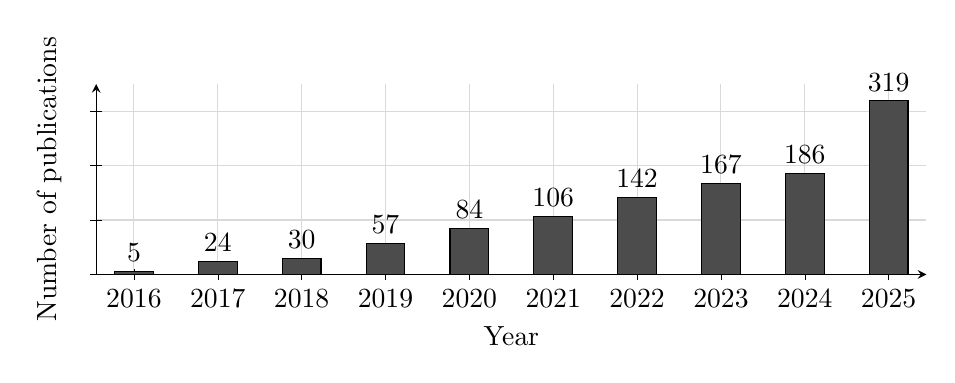
\begin{tikzpicture}
    \begin{axis}[
        width=\linewidth,
        height=4cm,
        ybar,
        bar width=14pt,
        ymin=0,
        ymax=350,
        yticklabels={},
        ylabel={Number of publications},
        xlabel={Year},
        symbolic x coords={2016,2017,2018,2019,2020,2021,2022,2023,2024,2025},
        nodes near coords,
        nodes near coords align={vertical},
        grid=both,
        major grid style={gray!30},
        minor grid style={gray!15},
        axis lines=left,
        tick style={black},
        enlarge x limits=0.05,
        title style={font=\bfseries},
    ]
    \addplot[
        fill=black!70
    ] coordinates {
        (2016,5)
        (2017,24)
        (2018,30)
        (2019,57)
        (2020,84)
        (2021,106)
        (2022,142)
        (2023,167)
        (2024,186)
        (2025,319)
    };
    \end{axis}
    \end{tikzpicture}
    }
    \caption{Yearly growth of Explainable Reinforcement Learning research with at least one citation on arXiv.}
    \label{fig:count_publications_xrl}
\end{figure}


This chapter presents the main existing \gls{xrl} methods.
We first define what is meant by an explanation in the context of \gls{xai}.
We then propose a taxonomy for organizing existing \gls{xrl} methods.
This taxonomy serves as the basis for the state-of-the-art review presented in the remainder of the chapter.

\section{Explanation in Artificial Intelligence}
\label{sec:explanation}

In this section, we define what an explanation is in the context of \gls{xai} and how it can be obtained.
We first introduce the concept of explanation in general, along with the explainability method used to produce it.
We then describe how this concept applies to \gls{xai}.
Finally, we further detail the properties that characterize an explainability method in the context of \gls{xai}.

\subsection{Explanation}
Establishing what is meant by an explanation is challenging due to the fundamentally multidisciplinary nature of the concept.
When we refer to explanation, we are inherently referring to an explanation provided to a human.
As soon as humans are involved, the problem is no longer purely computational or mathematical.
It involves several fields of research, such as philosophy, psychology, and sociology.
So far, these disciplines have not converged on a unified definition of explanation that can be directly applied to \gls{xai} \cite{miller2019explanation, bellucci2021towards}.

For this reason, we propose the following definition of explanation.
An explanation involves two entities: the object (Definition~\ref{def:object}) being explained and the receiver of the explanation.
The receiver is a human who aims to understand how the object operates and will be referred to as the observer throughout this manuscript (Definition~\ref{def:observer}).
The observer seeks to understand the object and, in doing so, builds a mental model of its functioning.
An explanation is therefore what allows the observer to refine and correct their mental model of how the object operates (Definition~\ref{def:explanation}).
This refinement is obtained through a transformation process that produces an explanation from the object being explained.
We refer to this process as an explainability method (Definition~\ref{def:explainability_method}), detailed further in Section~\ref{subsec:explainability_method}.

For an observer to understand an explanation, the information it contains must be interpretable (Definition~\ref{def:interpretable}).
Information is considered interpretable when it can be directly understood by a human without requiring any additional transformation process.

\begin{definition}{Object}{object}
The object of an explanation is the system the observer wants to understand.
\end{definition}

\begin{definition}{Observer}{observer}
The observer is the human who aims to understand an object.
The observer possesses a mental model of the object being explained.
This mental model is an internal representation of how the observer believes the system operates.
This representation may be incomplete or inaccurate.
\end{definition}

\begin{definition}{Interpretable}{interpretable}
Information is interpretable when it can be directly understood by an observer without requiring any additional transformation process.
\end{definition}

\begin{definition}{Explanation}{explanation}
An explanation is any interpretable information that enables an observer to refine or correct their mental model of the object of the explanation.
\end{definition}

\begin{definition}{Explainability Method}{explainability_method}
An explainability method is a transformation process that produces an explanation from the object being explained.
\end{definition}

This definition of explanation provides the foundation for the approach to explainability adopted throughout this manuscript.
Its generality allow it to encompass the different explainability methods considered in the following sections.

Moreover, this perspective avoids a binary interpretation of explainability, in which a system is considered either explainable or non-explainable.
The notion of a non-explainable system is difficult to justify from a scientific standpoint.
Scientific inquiry is driven by the assumption that observed phenomena can be investigated through the development of increasingly accurate analytical tools.
Declaring a system to be inherently impossible to explain would therefore conflict with this methodological principle.
This approach aligns with the philosophical Principle of Sufficient Reason, which states that every phenomenon rests upon an explainable basis \cite{sep-sufficient-reason}.

This quantitative perspective allows us to express an intuitive idea: not all explanations provide the same level of value \cite{doshivelez2017rigorous}.
The effectiveness of an explanation depends on its ability to improve the observer's understanding of the system.
For example, describing a marginal aspect of a system is different from correcting an observer's misunderstanding of a key mechanism.

\begin{figure}[t]
    \centering

    % --- Layout parameters --------------------------------------------
    % Horizontal distance between the centers of two consecutive blocks.
    \pgfmathsetmacro{\blockDistance}{6.6}
    % Width/height of each block (keep in sync with the node styles below).
    \pgfmathsetmacro{\blockSize}{3.6}
    % Fixed text width inside each block, so that longer labels wrap onto
    % extra lines (growing the block downward) instead of growing wider
    % and colliding with the neighboring block.
    \pgfmathsetmacro{\blockTextWidth}{3.1}
    % Text width used for the labels placed above/below the arrows.
    \pgfmathsetmacro{\arrowTextWidth}{2.6}

    % Vertical offset of the legend row below the main diagram.
    \pgfmathsetmacro{\legendYShift}{-3.6}
    % Horizontal offset of the start of the legend row (position of its first icon).
    \pgfmathsetmacro{\legendXShift}{-\blockSize/2 + 0}
    % Horizontal gap between two consecutive legend entries.
    \pgfmathsetmacro{\legendGap}{1.5}
    % Horizontal gap between a legend icon and its own label.
    \pgfmathsetmacro{\legendIconTextGap}{0.3}
    % --------------------------------------------------------------------

\resizebox{\textwidth}{!}{
\begin{tikzpicture}[]
% Nodes
\node[draw, rectangle, align=center, text width=\blockTextWidth cm, minimum width=\blockSize cm, minimum height=\blockSize cm] (box1) at (0, 0) {\hyperref[def:object]{\hl{\textbf{Object}}} \\ the system \\ the observer \\ seeks to understand};
\node[draw, rectangle, right of=box1, align=center, text width=\blockTextWidth cm, minimum width=\blockSize cm, minimum height=\blockSize cm] (box2) at (\blockDistance, 0) {\hyperref[def:explanation]{\hl{\textbf{Explanation}}} \\ \hyperref[def:interpretable]{\hl{interpretable}} \\ information enabling \\ the observer to refine \\ their mental model};
\node[draw, rectangle, right of=box2, align=center, text width=\blockTextWidth cm, minimum width=\blockSize cm, minimum height=\blockSize cm] (box3) at (2*\blockDistance, 0) {\textbf{Mental model} \\ of the observer \\ regarding the object};
% Arrows
\draw[-{Latex[length=3mm]}] (box1) -- node[midway, above, align=center, text width=\arrowTextWidth cm] {Information \\ extraction \\ through the use \\ of an \\ \hyperref[subsec:explainability_method]{\hl{\textbf{explainability}\\\textbf{method}}}} node[midway, below, align=center] {} (box2);
\draw[-{Latex[length=3mm]}] (box2) -- node[midway, above, align=center, text width=\arrowTextWidth cm] {\textbf{Interpretation} \\ by \\ the observer} node[midway, below, align=center] {} (box3);

% Legend: each entry is chained to the previous one via \legendGap /
% \legendIconTextGap, so the whole row reflows consistently if a label
% changes length or if the gaps are retuned.
\node[draw, rectangle, minimum width=0.3cm, minimum height=0.3cm] (legendIcon1) at (\legendXShift, \legendYShift) {};
\node[anchor=west, right=\legendIconTextGap of legendIcon1] (legendText1) {Information structures};

\node[inner sep=0pt, anchor=west, right=\legendGap of legendText1] (legendArrowStart) {};
\coordinate (legendArrowEnd) at ([xshift=0.4cm]legendArrowStart);
\draw[-{Latex[length=1.5mm]}] (legendArrowStart) -- (legendArrowEnd);
\node[anchor=west, right=\legendIconTextGap of legendArrowEnd] (legendText2) {Information transformation};

\node[anchor=west, right=\legendGap of legendText2] (legendIcon3) {\hl{~~}};
\node[anchor=west, right=\legendIconTextGap of legendIcon3] (legendText3) {Concepts discussed in more detail in this section};

% Brace: spans from just past box2 to just past box3, so it automatically
% follows \blockDistance and \blockSize instead of being retuned by hand.
\coordinate (C) at (\blockDistance+\blockSize/2+1, 2.6);
\coordinate (D) at (2*\blockDistance+\blockSize/2+1, 2.6);
\draw [decorate, decoration={brace, amplitude=10pt}, thick]
          (C) -- node[above=12pt, align=center] {Subjective analysis \\ by the \hyperref[def:observer]{\hl{observer}}} (D);
\end{tikzpicture}
    }
\caption{Explanation process in explainable artificial intelligence.}
\label{fig:explanation_process_illustration}
\end{figure}


Figure~\ref{fig:explanation_process_illustration} summarizes this whole explanation process, from the object of the explanation to the mental model refined by the observer, as a chain of three information structures, depicted as boxes and connected by arrows denoting a transformation of information:
\begin{enumerate}
    \item[(1)] The \textbf{object} of the explanation, that is, the system the observer seeks to understand.
    \item[(2)] The \textbf{explanation}, the interpretable information produced from the object.
    This transformation is performed through the use of an explainability method.
    \item[(3)] The \textbf{mental model} held by the observer regarding the object.
\end{enumerate}
A brace spanning boxes~(2) and~(3) indicates that this second half of the process, from the explanation to the resulting mental model, constitutes a subjective analysis carried out by the observer.

\subsection{Explainable Artificial Intelligence}

Now that the general framework of explanation has been established, we can examine how this concept applies in the context of \gls{ai}.
In the context of \gls{xai}, the object of explanation is an \gls{ai} system.
More precisely, \gls{xai} emerged as a response to the success of \gls{dl} models \cite{gunning2019darpa, arrieta2020explainable}.
In these architectures, information is represented in a distributed manner across the network through patterns of activation and connections between computational units.
Unlike symbolic approaches, individual components of \glspl{nn} cannot be directly associated with human-defined concepts.
From this starting point, we identify two types of approaches:
\begin{itemize}
    \item \textbf{Substitutive explainability:} In this approach, the underlying assumption is that there is nothing to explain within a \gls{nn}.
    There is no semantic meaning associated with each computational component, and therefore nothing to interpret.
    This corresponds to the so-called ``black box'' view of \glspl{nn}.
    Under this assumption, \gls{xai} consists of replacing as much of the \gls{dl} system as possible with alternative \gls{ai} methods \cite{rudin2019stop}.

    \item \textbf{Intrinsic explainability:} In this approach, it is argued that \glspl{nn} inherently contain mechanisms that can be explained.
    The limitation is considered to lie not in the networks themselves, but in the absence of adequate tools to analyze their functioning \cite{olah2020zoom}.
\end{itemize}

This manuscript considers methods from both approaches in order to provide a comprehensive overview of the \gls{xai} field.
According to the definition of explanation adopted in this manuscript (Definition~\ref{def:explanation}), we consider that any system can be explained.
As a consequence, the perspective adopted throughout this manuscript is that of intrinsic explainability.

\subsection{Explainability Method in XAI}
\label{subsec:explainability_method}

Now that the general framework of \gls{xai} has been established, we need to further detail the properties of an explanation in this context.
In our framework, an explanation in the field of \gls{xai} can be characterized by three components:
\begin{itemize}
    \item \textbf{Source:}\label{item:source} refers to the origin of the information used by the explainability method.
    The explainability method transforms the raw information produced by the \gls{ai} system into an explanation that can be understood by an observer.

    \item \textbf{Form:}\label{item:form} refers to the representation through which the explanation is communicated.
    The form defines how the information is presented to the observer and must allow human interpretation.
    An explanation can take many different forms, including text, images, computer code, and mathematical equations.

    \item \textbf{Subject:}\label{item:subject} refers to the aspect of the \gls{ai} system that is being explained.
    In \gls{xai}, this distinction is commonly associated with the difference between local and global explanations.
    A local explanation describes why an \gls{ai} system produced a specific output in a given situation.
    A global explanation aims to describe the general functioning of the \gls{ai} system.
\end{itemize}

These three properties of an explanation are entirely determined by the explainability method (Definition~\ref{def:explainability_method}) used to produce it.
In this context, an explainability method is a transformation process that maps a source of information into an explanation characterized by a specific form and subject.
Research in \gls{xai} focuses on developing new methods capable of performing this transformation in order to overcome the lack of interpretability associated with \gls{dl} models.
\section{Taxonomy of XRL Methods}
\label{sec:taxonomy_xrl_methods}

Now that the concept of \gls{xai} has been defined, we turn to its application in \gls{rl}, known as \gls{xrl}.
As in \gls{xai}, explanations in \gls{xrl} are produced by explainability methods and can be described in terms of their subject, source, and form.
This section reviews the possible variations of these three aspects in the specific context of \gls{rl}.

\subsection{Subject}
\label{subsec:subject}

The first question to address is the subject of explanation in the context of \gls{rl}.
To answer this question, it is necessary to identify the different components involved in a \gls{rl} system and determine which of them constitutes the object of explanation.
A \gls{rl} system can be described through two main components: the environment and the policy.

The environment defines the dynamics in which the agent evolves, including the possible states, observations, actions, and transitions.
Environments are simulations designed by humans, and their dynamics are explicitly defined.
Therefore, it is assumed that the environment is known to the observer and does not require explanation.

The main object of interest is therefore the agent's policy.
The policy represents the decision-making mechanism of the agent.
It is a function that maps observations to actions and is learned through interaction with the environment in order to maximize the expected cumulative reward.
The policy is the component that encodes the learning process and that \gls{xrl} aims to explain.

Explaining a policy introduces additional challenges compared with classical \gls{xai} settings.
In traditional \gls{xai} problems, the objective is to explain an isolated decision, such as determining which features of an image led to a classification result.
In contrast, \gls{rl} introduces a temporal dimension into the decision-making process.
An action is not only determined by the current observation but also influences future states and rewards.
Therefore, understanding the behavior of an agent may require considering a sequence of interactions between the agent and its environment.

This temporal dimension leads to a distinction between two objectives of explanation in \gls{xrl}:
\begin{itemize}
    \item \textbf{Decision explanations:} focus on identifying the elements of the current observation that influenced the action selected by the policy.
    This type of explanation is close to classical \gls{xai} approaches, as it analyzes the relationship between inputs and outputs while abstracting away the sequential nature of the decision process.

    \item \textbf{Strategy explanations:} aim to characterize the agent's behavior over time.
    They focus on sequences of decisions and interactions with the environment in order to understand how the agent achieves its long-term objective.
    This type of explanation is specific to \gls{rl}, as it addresses the temporal and goal-oriented nature of the learning process.
\end{itemize}

These two objectives should not be considered as strictly separated categories, but rather as two extremes of a continuum.
Indeed, understanding the elements of an observation that influence a specific decision can help the observer generalize this information to infer broader aspects of the agent's behavior.
Conversely, understanding the agent's overall strategy can provide insights into the reasoning behind individual decisions.

\subsection{Source}
\label{subsec:source}

We identify three sources of explanation in \gls{rl}, all obtained during or after the learning process and containing information about the agent:
\begin{itemize}
    \item \textbf{Policies:} policies are functions that generate a distribution over the action space for a given observation.
    The objective of \gls{rl} is to learn a policy that maximizes the expected cumulative future rewards.
    During the learning phase, the policy is iteratively improved through interactions with the environment.

    \item \textbf{Trajectories:} trajectories represent sequences of successive interactions between the agent and the environment.
    At each step, the agent selects an action based on its observation, which modifies the environment and produces a reward as well as a new observation.
    This process continues until the end of the trajectory.

    \item \textbf{Value functions:} value functions provide predictions about the future outcome of a trajectory from a given observation.
    The most commonly used value function is the critic function, which estimates the expected sum of future rewards.
    This prediction guides the learning process, as the agent updates its policy to maximize the estimated future return.
    However, other types of value functions can also be used as sources of explainability.
\end{itemize}

\subsection{Form}
\label{subsec:form}

We identify six forms of explanation in the \gls{rl} setting:
\begin{itemize}
    \item \textbf{Policy Model:} an interpretable model of the agent's policy function.
    
    \item \textbf{Saliency Map:} a weighting of the input features representing their influence on the output of the policy function.
    
    \item \textbf{Counterfactual:} a modified observation obtained by perturbing the original observation in order to produce a different action from the agent.
    
    \item \textbf{Agent Trajectory:} a sequence of successive interactions between the agent and the environment.
    
    \item \textbf{Trajectory Prediction:} a prediction about the future evolution of the trajectory produced by a value function.
    
    \item \textbf{Interaction Model:} an interpretable model of the interactions between the agent and the environment.
\end{itemize}

Among the three components characterizing an explanation, the form is the one that varies most significantly across explainability methods.
While subjects and sources tend to be relatively stable in the \gls{xrl} literature, the diversity in how explanations are presented is considerably greater.
The list above is by no means definitive and may evolve as new approaches emerge.
For this reason, the following section is organized according to the form of explanations and presents existing explainability methods based on this criterion.

\section{State-of-the-Art Review of XRL Methods}
\label{sec:state_of_the_art}
\begin{table*}[t]
% \footnotesize
\hspace*{\fill}
\resizebox{\textwidth}{!}{
\begin{tblr}{|Q[c,m]|Q[c,m,4cm]|Q[c,m,7cm]|Q[c,m]|Q[c,m]|Q[c,m]|}
    \hline
    \SetCell[r=2]{c} \hyperref[subsec:subject]{\textbf{Explanation \\ Target}} & \SetCell[r=2]{c} \hyperref[subsec:form]{\textbf{Explanation \\ Form}} & \SetCell[r=2]{c} \hyperref[sec:state_of_the_art]{\textbf{Explainability \\ Method}} & \SetCell[c=3]{} \hyperref[subsec:source]{\textbf{Source of \\ Explanation}} & & \\
    \hline
    & & & \rotatebox{-90}{\shortstack{Policy}} & \rotatebox{-90}{\shortstack{Trajectories}} & \rotatebox{-90}{\shortstack{Value \\ functions}} \\
    \hline
    \hline
    \SetCell[r=6]{c} Decision & \SetCell[r=2]{c} \hyperref[subsec:policy_model]{{Policy Model}} & \hyperref[subsubsec:interpretable_policy_learning]{{\textit{Interpretable policy learning}}} & \scalebox{2}{\checkmark} & & \\
    \hline
    & & \hyperref[subsubsec:policy_approximation_via_interpretable_model]{{\textit{Policy approximation via interpretable model}}} & \scalebox{2}{\checkmark} & & \\
    \hline
    & \SetCell[r=3]{c} \hyperref[subsec:saliency_map]{{Saliency Map}} & \hyperref[subsubsec:observation_perturbation]{\textit{Observation perturbation}} & \scalebox{2}{\checkmark} & & \\
    \hline
    & & \hyperref[subsubsec:observation_gradient_analysis]{\textit{Observation gradient analysis}} & \scalebox{2}{\checkmark} & & \\
    \hline
    & & \hyperref[subsubsec:attention_based_architecture]{\textit{Attention-based architecture}} & \scalebox{2}{\checkmark} & & \\
    \hline
    & \hyperref[subsec:counterfactual]{{Counterfactual}} & \hyperref[subsubsec:latent_space_counterfactual_generation]{\textit{Latent space usage for counterfactual generation}} & \scalebox{2}{\checkmark} & & \\
    \hline
    \hline
    \SetCell[r=7]{c} Strategy & \SetCell[r=2]{c} \hyperref[subsec:trajectory_prediction]{{Trajectory Prediction}} & \hyperref[subsubsec:value_functions_as_observations]{{\textit{Value functions as observations}}} & & & \scalebox{2}{\checkmark} \\
    \hline
    & & \hyperref[subsubsec:critic_enrichment]{\textit{Critic enrichment}} & & & \scalebox{2}{\checkmark} \\
    \hline
    & \SetCell[r=2]{c} \hyperref[subsec:interaction_model]{{Interaction Model}} & \hyperref[subsubsec:bayesian_network_learning]{\textit{Bayesian network learning}} & & \scalebox{2}{\checkmark} & \\
    \hline
    & & \hyperref[subsubsec:latent_space_mdp_generation]{{\textit{Latent space usage for MDP generation}}} & \scalebox{2}{\checkmark} & & \\
    \hline
    & \SetCell[r=3]{c} \hyperref[subsec:agent_trajectory]{{Agent Trajectory}} & \hyperref[subsubsec:hierarchical_decomposition]{\textit{Hierarchical decomposition}} & \scalebox{2}{\checkmark} & & \\
    \hline
    & & \hyperref[subsubsec:extraction_via_critic_analysis]{\textit{Extraction via critic analysis}} & & \scalebox{2}{\checkmark} & \scalebox{2}{\checkmark} \\
    \hline
    & & \hyperref[subsubsec:extraction_via_multi_critic_comparisons]{\textit{Extraction via multi-critic comparisons}} & & \scalebox{2}{\checkmark} & \scalebox{2}{\checkmark} \\
    \hline
\end{tblr}
}
\hspace*{\fill}
\caption{Taxonomy of explainability methods in reinforcement learning.}
\label{tab:taxonomy_methods}
\end{table*}


The purpose of this section is to detail the functioning of existing explainability methods (see Table~\ref{tab:taxonomy_methods}).
They are presented according to the form of explanation they produce, following the taxonomy introduced in Section~\ref{sec:taxonomy_xrl_methods}.

Each subsection introduces one of the six forms of explanation identified in Section~\ref{subsec:form}.
For each form, we identify the corresponding family of methods and organize the related approaches within the appropriate subsection.
A family of methods is defined as a set of methods that share the same source, form, and subject of explanation, as well as a similar procedure for generating explanations.
Methods belonging to the same family may differ slightly in their implementation or in the details of the generation process.
They share a common underlying principle that allows them to be described as part of the same family.

\subsection{Policy Model}
\label{subsec:policy_model}

The policy function can be represented by a wide variety of function classes.
In modern reinforcement learning, neural networks is the most commonly used models for representing policies.
Although these models achieve the highest performance, their connectionist nature makes their internal representations non-interpretable.

For this reason, a substitutive approach to XRL aims to replace these models with alternative models considered interpretable.
Such models can be understood through direct analysis of their representations.
The main classes of interpretable models used to represent policy functions include decision trees \cite{topin2021iterative}, algorithms \cite{trivedi2022learning}, formal logic \cite{payani2019inductive}, and linear models \cite{pmlr-v108-garreau20a}.

Explanations derived from an interpretable model primarily provide insights into the decision-making process, since what is modeled is the mapping between an observation and an action.
If the model is sufficiently simple or well structured, the observer can form a mental representation of a sequence of decisions across the environment and thus obtain information about the agent's strategy.

The main limitation of these methods is that interpretable models rely on symbolic representations.
When the policy to be represented is too complex, achieving comparable performance requires a large number of rules or conditions.
The resulting model can quickly become difficult to analyze and lose its interpretability.


For example, representing a policy capable of playing Go using a symbolic model would require considering a very large number of possible situations and specific cases.
Even if such a representation were possible, the resulting model would likely become intractable for human analysis due to its complexity.
This illustrates why neural network-based approaches have become dominant in such domains, as they can learn complex decision strategies without requiring an explicit enumeration of rules.

To obtain an interpretable policy model, two explainability methods are available: \textit{interpretable policy learning} and \textit{policy approximation via interpretable model}.

\subsubsection{\textit{Interpretable Policy Learning}}
\label{subsubsec:interpretable_policy_learning}

This method aims at learning a policy represented by an \textbf{interpretable} model \cite{topin2021iterative, trivedi2022learning}.
It is the most direct approach to addressing the challenges posed by explainable reinforcement learning (XRL).
This type of training requires modifying the MDP in order to adapt it to the search space and to the type of policy representation.
Moreover, this search space often needs to be reduced to make learning feasible.
Such a \textbf{reduction} requires the integration of \textbf{expert knowledge} into the learning process.
With this method, the \textit{interpretable policy function} itself is used to provide explanations to the observer.

\subsubsection{\textit{Policy Approximation via Interpretable Model}}
\label{subsubsec:policy_approximation_via_interpretable_model}

Using an interpretable model, it is possible to \textbf{approximate} a non-interpretable policy \cite{sieusahai2021explaining}.
In this setting, the problem is cast as a \textbf{supervised learning} task, where the non-interpretable policy is used to label each observation with the action it selects.
Using this dataset, supervised learning is then performed with the interpretable model.
The resulting \textit{interpretable model} is subsequently used as an explanation for the observer.
If this approximation is sufficiently faithful, it can be deployed in the environment in place of the original policy, thereby enabling a high degree of control over the agent.

\subsection{Saliency Map}
\label{subsec:saliency_map}

\begin{figure}[t]
    \centering
    \begin{subfigure}[b]{0.4\textwidth}
        \centering
        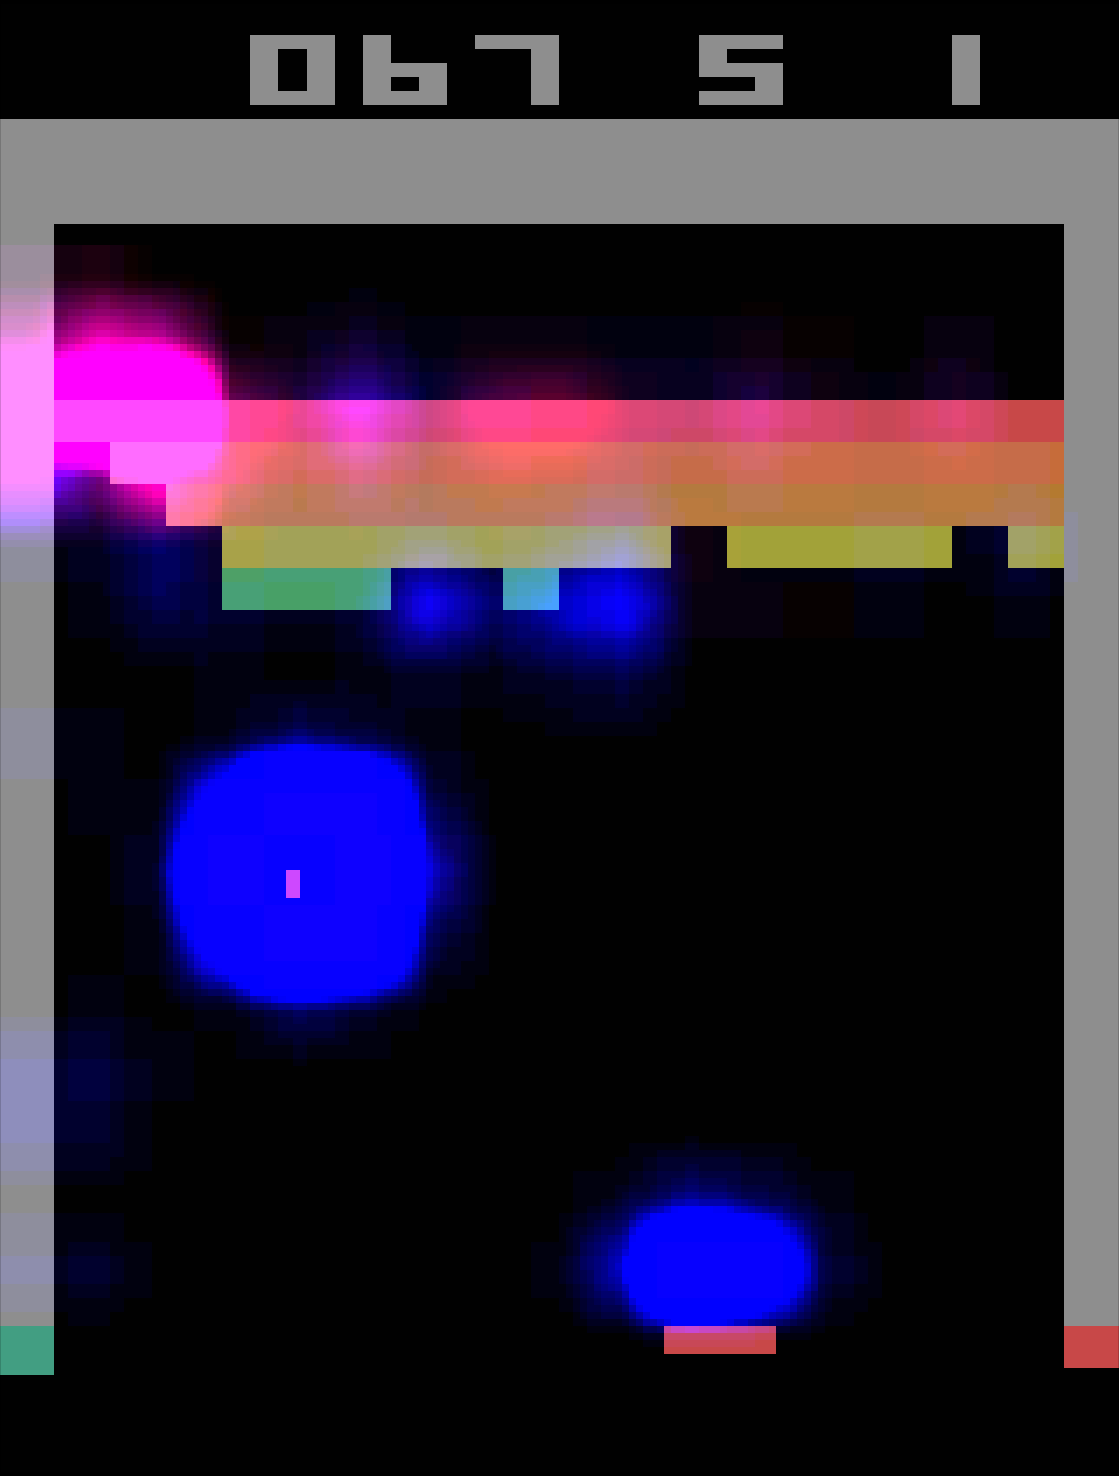
\includegraphics[width=\textwidth]
            {figures/explainability_reinforcement_learning/hit_map_1.png}
        \caption{}
        \label{fig:saliency_map_heatmap_perturbation}
    \end{subfigure}
    \hspace{0.02\textwidth}
    \begin{subfigure}[b]{0.4\textwidth}
        \centering
        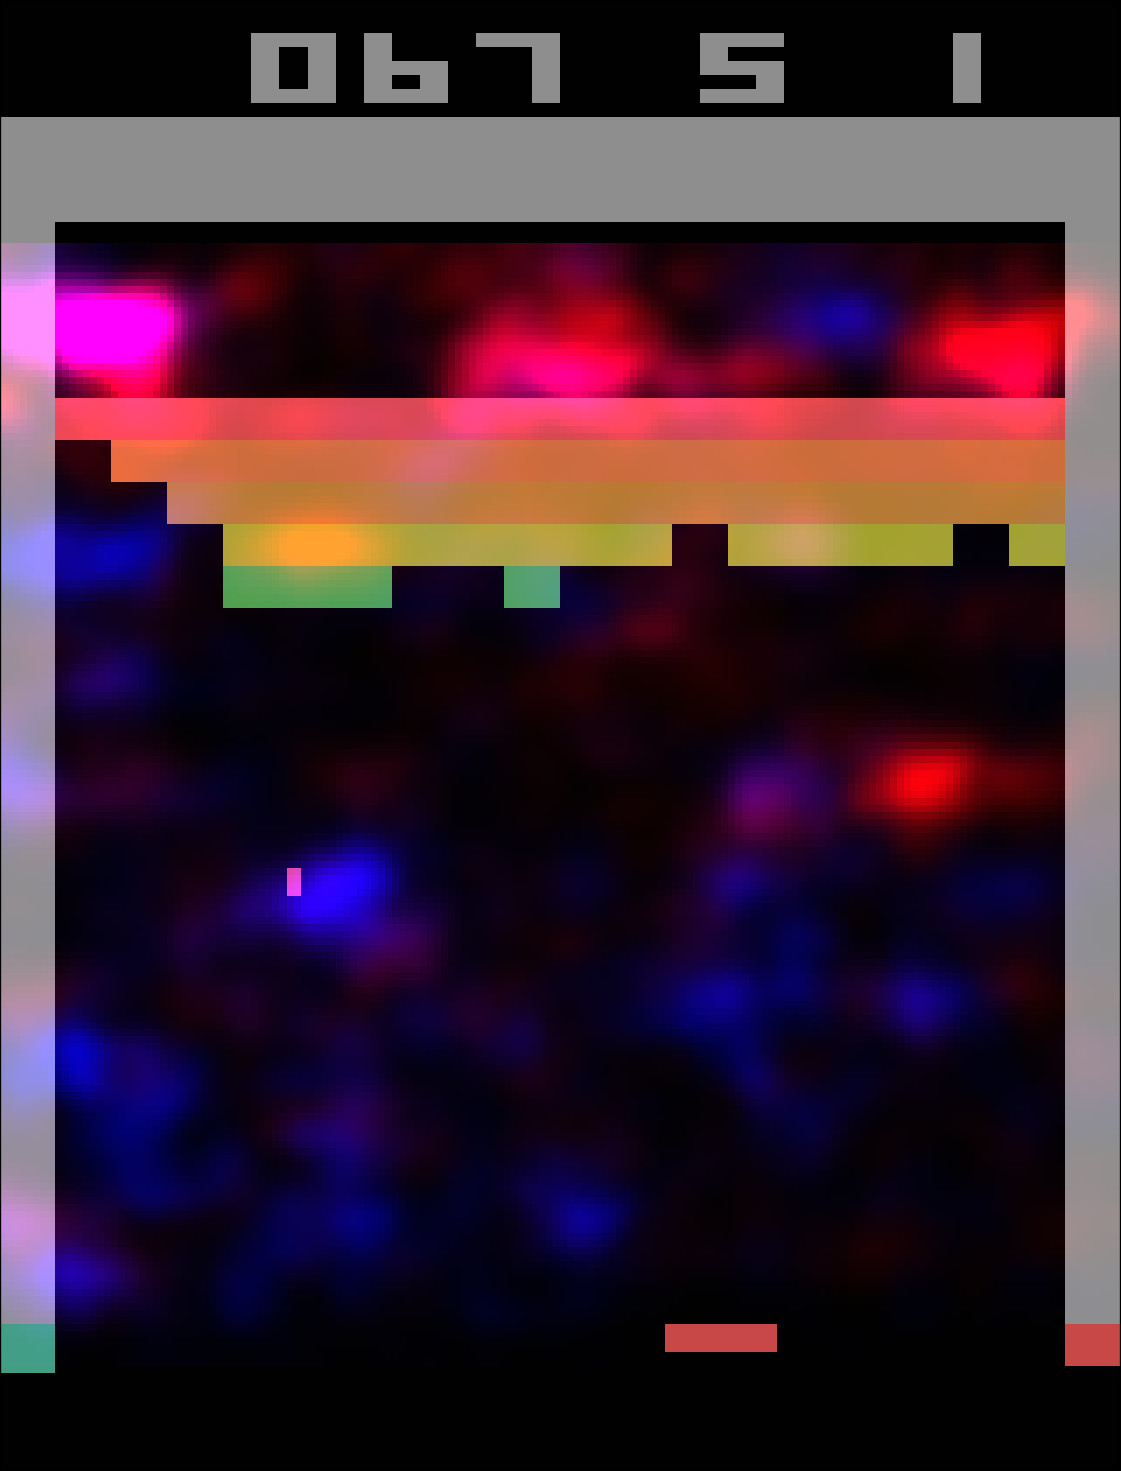
\includegraphics[width=\textwidth]
            {figures/explainability_reinforcement_learning/hit_map_2.png}
        \caption{}
        \label{fig:saliency_map_heatmap_gradient}
    \end{subfigure}
    \caption{
        Heatmaps for the same observation of the Atari game ``Breakout'' \cite{greydanus2018visualizing}.
    }
    \label{fig:saliency_map_heatmap}
\end{figure}


Heatmaps make it possible to identify which parts of the input vector are decisive in the selection of the output (as illustrated in Figure~\ref{fig:saliency_map_heatmap}).
When applied to the reinforcement learning setting, they highlight the regions of the observation space that are critical in the action selection process.
By nature, this form of explanation provides information about the policy's decision-making process.
The intuitive nature of this representation allows it to be used by a broad audience.

A limitation of heatmap-based methods is that the resulting explanations are not always directly meaningful to the observer.
As illustrated in Figure~\ref{fig:saliency_map_heatmap_gradient}, interpreting which regions are important often requires human reasoning and involves a degree of subjectivity.
This limitation becomes particularly relevant in reinforcement learning, where the objective is not only to explain a single decision but also to understand the factors influencing a sequence of decisions over time.

More generally, heatmap-based methods highlight a fundamental challenge in XAI: determining the relevance of an explanation.
Different methods can produce different heatmaps for the same decision, raising the question of how to compare and select among potentially conflicting explanations.
This is illustrated in Figure~\ref{fig:saliency_map_heatmap}, where the perturbation-based method (Figure~\ref{fig:saliency_map_heatmap_perturbation}) and the gradient-based method (Figure~\ref{fig:saliency_map_heatmap_gradient}) produce different heatmaps for the same observation.
Rather than assuming that only one explanation can be valid, the definition of explanation adopted in this manuscript allows for multiple complementary perspectives.
Different explanations may reveal different aspects of the system and contribute to improving the observer's understanding.

Three explainability methods can be used to obtain this type of explanation: \textit{observation perturbation}, \textit{observation gradient analysis}, and \textit{attention-based architectures}.

\subsubsection{\textit{Observation Perturbation}}
\label{subsubsec:observation_perturbation}

Perturbation analysis consists in applying various \textbf{modifications} to the observation in order to study their \textbf{impact} on the output of the \textbf{policy function} \cite{greydanus2018visualizing}.
The greater the variation in the output caused by a perturbation applied to a given component of the input vector, the higher the \textbf{weight} assigned to that component.
The magnitude of the perturbation is measured by computing the distance between the original output and the output obtained from the perturbed input.
Using this set of weights, a \textit{heatmap} is constructed, enabling the observer to visualize which parts of the observation vector are most sensitive in the action-selection process (see Figure~\ref{fig:saliency_map_heatmap_perturbation}).

\subsubsection{\textit{Observation Gradient Analysis}}
\label{subsubsec:observation_gradient_analysis}

Observation \textbf{gradient} analysis refers to a set of methods that require a differentiable policy function in order to extract information from it \cite{simonyan2014deep, weitkamp2019visual, huber2019enhancing}.
To this end, the gradient of the policy function is computed with respect to all \textbf{components of the input vector}.
For each input component, the resulting gradient provides a weighting that represents its importance in the output of the policy function.
Based on these weightings, a \textit{heatmap} is constructed to allow the observer to visually identify the parts of the input vector that are the most influential in the policy function's output (see Figure~\ref{fig:saliency_map_heatmap_gradient}).

\subsubsection{\textit{Attention-Based Architecture}}
\label{subsubsec:attention_based_architecture}

\begin{figure}[t]
    \centering
    \begin{subfigure}[b]{0.4\textwidth}
        \centering
        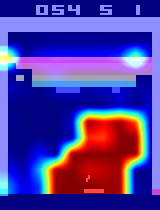
\includegraphics[width=\textwidth]
            {figures/explainability_reinforcement_learning/attention_map_1.png}
        \caption{}
        \label{fig:attention_map_heatmap_clear}
    \end{subfigure}
    \hspace{0.02\textwidth}
    \begin{subfigure}[b]{0.4\textwidth}
        \centering
        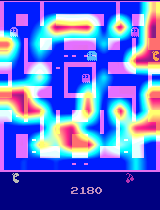
\includegraphics[width=\textwidth]
            {figures/explainability_reinforcement_learning/attention_map_2.png}
        \caption{}
        \label{fig:attention_map_heatmap_unclear}
    \end{subfigure}
    \caption{
        Attention-based heatmaps for the Atari games ``Breakout'' and ``Ms.\ Pac-Man'' \cite{mott2019towards}.
    }
    \label{fig:attention_map_heatmap}
\end{figure}


\textbf{Attention} blocks constitute a neural network architecture that makes it possible to weight the relative importance of one part of a vector with respect to the other parts of the same vector \cite{vaswani2023attention}.
These weights are computed as a function of the vector itself and are learned by the neural network during training.
For a given observation, each component of the observation vector is assigned a scalar value.
It can therefore be assumed that the components associated with the highest weights are the most influential in determining the output \cite{mott2019towards, itaya2021visual}.
This attention-based \textit{heatmap} is then provided to the observer as the explanation (see Figure~\ref{fig:attention_map_heatmap_clear}).
However, as shown in Figure~\ref{fig:attention_map_heatmap_unclear}, the attention weights are not always concentrated on a small, easily interpretable set of regions, which can make this type of explanation difficult to exploit.

\subsection{Counterfactual}
\label{subsec:counterfactual}

\begin{figure}[t]
    \centering
    \begin{subfigure}[b]{0.35\textwidth}
        \centering
        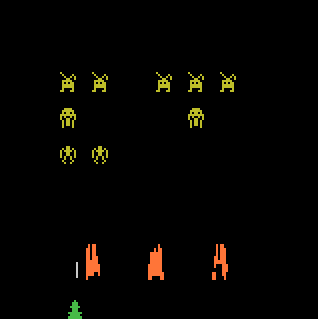
\includegraphics[width=\textwidth]
            {figures/explainability_reinforcement_learning/contrefactuel_1.png}
        \caption{}
        \label{fig:counterfactual_example_original}
    \end{subfigure}
    \hspace{0.02\textwidth}
    \begin{subfigure}[b]{0.35\textwidth}
        \centering
        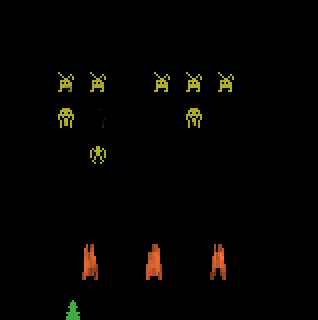
\includegraphics[width=\textwidth]
            {figures/explainability_reinforcement_learning/contrefactuel_2.png}
        \caption{}
        \label{fig:counterfactual_example_counterfactual}
    \end{subfigure}
    \caption{
        Counterfactual explanation of the agent's behavior for the Atari game \textit{Space Invaders} \cite{olson2021counterfactual}.
        Panel~\subref{fig:counterfactual_example_original} shows the original observation and panel~\subref{fig:counterfactual_example_counterfactual} the counterfactual observation produced by a generative model.
    }
    \label{fig:counterfactual_example}
\end{figure}


In the context of reinforcement learning, counterfactual explanations are used to generate new observations (see Figure~\ref{fig:counterfactual_example}).
This new observation, distinct from the original one, leads the agent to adopt an alternative behavior.
A counterfactual explanation aims to explain the agent's decision-making process.
Modifying the observation informs the observer about the adjustments required for the agent to adopt a different behavior.
The method available to generate counterfactuals is the \textit{use of the latent space for counterfactual generation}.

\subsubsection{\textit{Latent Space Usage for Counterfactual Generation}}
\label{subsubsec:latent_space_counterfactual_generation}

In this method, \textbf{generative models} are used \cite{bond2021deep} to exploit the latent representation.
This type of model learns to generate new data by imitating the training data distribution.
In this context, generative models aim to produce alternative observations that are likely to alter the agent's actions \cite{olson2021counterfactual}.

The main challenge of this approach lies in the fact that, to serve as explanations, counterfactuals must be both \textbf{close} and \textbf{feasible}.
A close counterfactual refers to one that does not differ significantly from the original observation.
A feasible counterfactual corresponds to an observation that is meaningful within the considered environment.

\subsection{Agent Trajectory}
\label{subsec:agent_trajectory}

Trajectories represent a sequence of interactions between the agent and its environment.
By analyzing these trajectories, the observer can infer the underlying dynamics governing the agent's evolution within its environment.

Post-training trajectories are systematically used to obtain explanations of the agent's strategy, even outside the scope of explainable reinforcement learning (XRL).
This simple approach can be enhanced using methods such as \textit{hierarchical decomposition} and \textit{extraction via critic analysis}.

Training trajectories, on the other hand, can be used to explain the agent's learning process, through the \textit{extraction via multi-critic comparisons} method.

\subsubsection{\textit{Hierarchical Decomposition}}
\label{subsubsec:hierarchical_decomposition}

Hierarchical agents are composed of a set of \textbf{sub-policies} specialized for specific tasks within subsets of the environment's states.
This method distributes the optimization of the reward function across multiple models, significantly simplifying the learning process.
Moreover, this \textbf{decomposition} of the policy function can also provide explainability in the agent's strategy \cite{Beyret_2019}.
If a sub-policy is selected, it indicates that the agent will execute a specialized behavior.
This behavioral specialization provides insight into the strategy the agent employs to maximize the reward function.
The agent's \textit{trajectory}, together with the \textit{sub-policy} selected for each action, is used as interpretable information.

\subsubsection{\textit{Extraction via Critic Analysis}}
\label{subsubsec:extraction_via_critic_analysis}

In this method, the predictions of the critic are used to determine which \textbf{trajectories to present to the observer} \cite{Sequeira_2020}.
A set of states is selected from multiple trajectories.
For a given state, all possible actions are examined.
The state is assigned a value equal to the difference between the critic's prediction for the lowest-valued action and the prediction for the highest-valued action.
Trajectories containing the states with the highest values according to this procedure are then chosen to be presented to the observer.
These trajectories are considered \textbf{critical moments} of the agent and are therefore relevant for analysis.
For this method, the \textit{selected trajectories} represent the interpretable information provided to the observer.

\subsubsection{\textit{Extraction via Multi-Critic Comparisons}}
\label{subsubsec:extraction_via_multi_critic_comparisons}

In this approach, the main objective is to \textbf{weight the training interactions} between the agent and the environment according to their influence on the learning process.
To achieve this, multiple critic functions are created using \textit{off-policy} learning.
Off-policy learning is a reinforcement learning process that allows a policy to learn from data generated by a different policy \cite{gottesman2020interpretable}.
Each critic function is trained on a subset of the dataset.

A reference critic function is trained using the entire dataset.
Then, for each agent-environment interaction, a critic function is retrained while specifically excluding that interaction.
The \textbf{prediction disparity} between the retrained critic and the reference critic represents the impact of removing that interaction on learning.
Through this procedure, a value is assigned to each interaction based on this difference: the larger the disparity, the higher the value assigned to the interaction.

A higher value indicates that the interaction is considered more important in the learning process.
These \textit{values} over the \textit{interactions} serve as explanations for the observer, providing a means to assess the significance of each agent-environment interaction within the learning process.

\subsection{Trajectory Prediction}
\label{subsec:trajectory_prediction}

\begin{figure}[t]
    \centering
    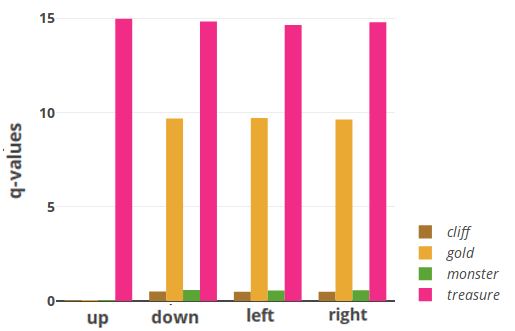
\includegraphics[width=0.6\textwidth]
        {figures/explainability_reinforcement_learning/multi_q_values.png}
    \caption{
        Prediction of sub-rewards as a function of the action selected by the
        agent for a given state \cite{juozapaitis2019explainable}. Depending
        on the action chosen by the agent, one can determine which
        sub-reward it aims to maximize.
    }
    \label{fig:trajectory_prediction_values}
\end{figure}


Making predictions about the future of a trajectory allows one to form a representation of what the system expects, based on its training experience (see Figure~\ref{fig:trajectory_prediction_values}).
These predictions are produced using value functions.
Such functions provide insights into the future evolution of the agent's trajectory.
By their nature, this form of explanation informs the observer about the strategy adopted by the agent.

The main challenge of this type of approach lies in ensuring that the values predicted by these functions are truly decisive in the actions selected by the agent.
To this end, the following methods are employed: \textit{value functions as observations} and \textit{critic enrichment}.

\subsubsection{\textit{Value Functions as Observations}}
\label{subsubsec:value_functions_as_observations}

The objective is to train \textbf{interpretable value functions} to be used as observations for the agent.
If the features predicted by these value functions are \textbf{meaningful} to the observer, they can determine which aspects the agent is attempting to maximize through its actions \cite{lin2021contrastive}.

\subsubsection{\textit{Critic Enrichment}}
\label{subsubsec:critic_enrichment}

In order to obtain interpretable information from the predictions of the \textbf{critic}, it is possible to \textbf{decompose} the critic into multiple \textbf{sub-functions} \cite{juozapaitis2019explainable}.
The reward function is thus decomposed into multiple sub-reward functions, each representing a \textbf{sub-objective} of the task to be accomplished.
Similarly, for each of these sub-reward functions, corresponding sub-critic functions are defined, along with a function that combines their outputs.
During training, the agent selects its actions so as to maximize this combination function of the sub-critics.
Using this approach, for each observation and action, a prediction is obtained regarding the sub-objectives the agent is attempting to maximize.
This \textit{prediction} is then used as the explanation for the observer.

\subsection{Interaction Model}
\label{subsec:interaction_model}

\begin{figure}[t]
    \centering
    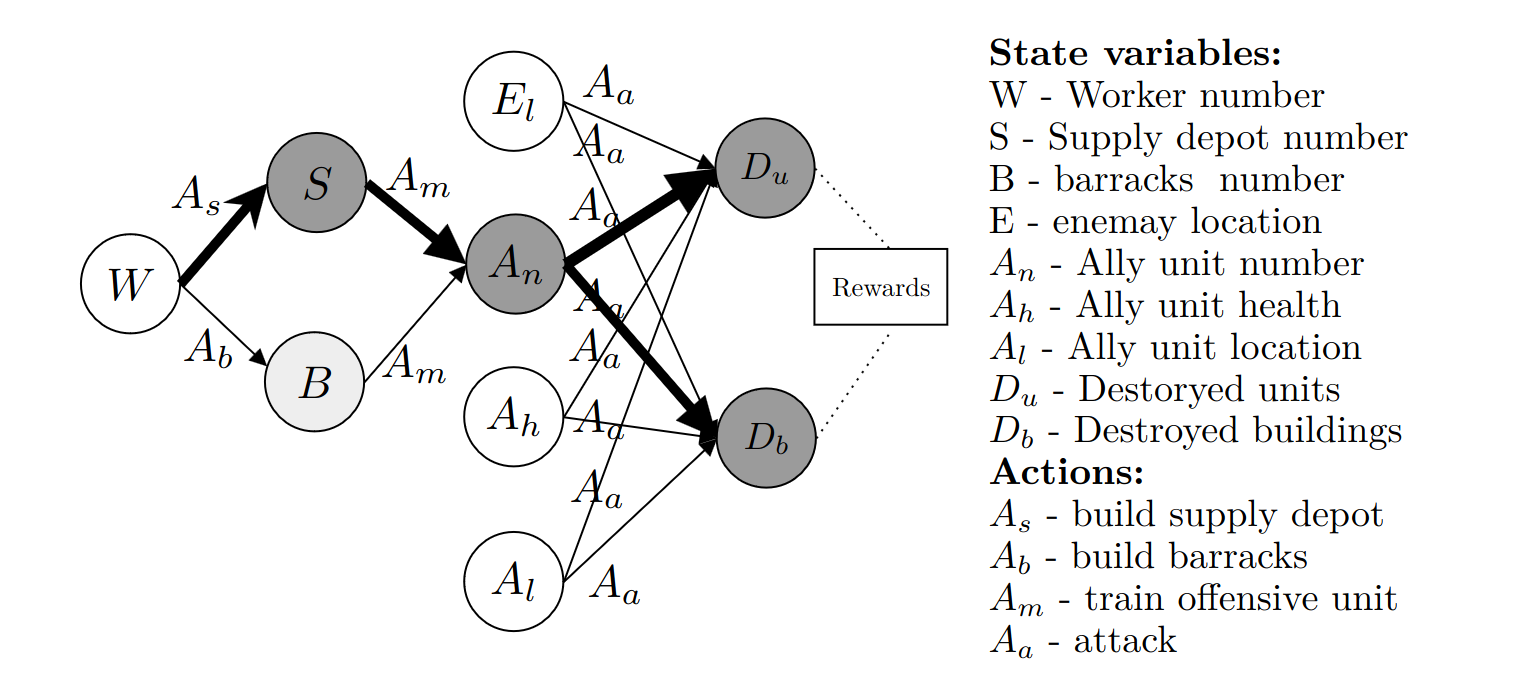
\includegraphics[width=0.9\textwidth]
        {figures/explainability_reinforcement_learning/graph_causal.png}
    \caption{
        Agent--environment interaction model for the video game \textit{StarCraft II} \cite{madumal2020explainable}.
    }
    \label{fig:interaction_model_causal_graph}
\end{figure}


Modeling the interactions between an agent and its environment makes it possible to understand how the agent's decisions are made and what impact they have on the environment (see Figure~\ref{fig:interaction_model_causal_graph}).
By incorporating these interactions into an explanatory model, one can better grasp the complex relationships between the agent and its environment, thereby identifying the determining factors in the decision-making process.
By explicitly handling the agent--environment interaction, this type of explanation aims to explain the agent's strategy.
The methods used to obtain explanations in the form of agent--environment interactions are: \textit{Bayesian network learning} and \textit{latent space usage for MDP generation}.

\subsubsection{\textit{Bayesian Network Learning}}
\label{subsubsec:bayesian_network_learning}

The evolution of an agent within an environment can be observed as a set of \textbf{random variables} connected through a \textbf{Bayesian network} \cite{madumal2020explainable}.
Random variables are defined to represent both external aspects (the environment) and internal aspects of the agent (the actions).
By analyzing trajectories, it becomes possible to infer causal relationships among these random variables.
At the end of this process, a weighted causal graph is obtained, which serves as an explanation for the observer.
This \textit{Bayesian network}, representing the interactions between the agent and the environment, is then used as the explanation.

\subsubsection{\textit{Latent Space Usage for MDP Generation}}
\label{subsubsec:latent_space_mdp_generation}

Each layer of a neural network can be viewed as a projection from one space to another \cite{zahavy2017graying}.
As information propagates through successive layers of a neural network, it becomes increasingly abstract.
It can therefore be assumed that two vectors that are close in this projected space are also close in terms of the agent's perception.
Based on this observation, it is possible to \textbf{redefine an MDP} by leveraging the \textbf{abstract representations} produced by the final layers of a neural network.
Once the new MDP has been constructed, a model of the interaction between the agent and its environment is obtained.
This model, represented as a \textit{graph}, is then used as the explanation.

\section{Conclusion}
\label{sec:explainability_reinforcement_learning_conclusion}

The taxonomy and the state-of-the-art review presented in this chapter make it possible to draw three main observations.

\subsection{Absence of Explanation of the Learning Process}

First, regarding the subject of explanation, Table~\ref{tab:taxonomy_methods} shows that none of them addresses the learning process itself.
An explanation of the learning process in \gls{rl} would concern how the policy is progressively updated throughout training.
More specifically, it would aim to explain why the agent how this policy evolves over successive learning iterations and converges toward a particular policy.
We identify several reasons for this absence.

Among the different machine learning paradigms, \gls{rl} is the one that would benefit the most from explanations of the learning process.
Unlike supervised or unsupervised learning, \gls{rl} relies on an explicit exploration--exploitation trade-off, making the learning trajectory itself an informative object of explanation.
However, most \gls{xrl} methods are inherited from the XAI literature, where explanations almost exclusively focus on the behavior of already-trained models.
As a result, this limitation has naturally carried over to \gls{xrl}.

From a practical perspective, explaining the learning process is also of limited industrial interest.
In most real-world applications, practitioners deploy an already-trained agent, while the training phase takes place offline.
Users are generally interested in understanding the behavior of the final policy rather than the optimization process that produced it.

Finally, explaining the learning process raises significant methodological challenges.
Training in \gls{rl} can be viewed as the iterative improvement of a policy through repeated interactions with the environment.
In this sense, explaining learning would amount to explaining the evolution of a sequence of policies rather than a single one.
Given that current \gls{xrl} methods still struggle to provide comprehensive explanations of an individual policy, extending such explanations to an entire training trajectory appears considerably more difficult.
This suggests that explanations of the learning process remain an open research direction rather than an immediate extension of existing \gls{xrl} methods.

\subsection{Lack of Unified Metrics for Explainability}

Second, the diversity of explanation forms identified in this review reveals another limitation shared by nearly all families of \gls{xrl} methods: the absence of reliable metrics for evaluating explainability.
In many studies, explanations are not evaluated with human participants.
Authors focus on the technical properties of the proposed method, such as fidelity, sparsity, or computational efficiency.
When human evaluations are conducted, they usually rely on subjective satisfaction questionnaires.
Although useful, self-reported satisfaction is prone to numerous biases and does not necessarily indicate that the explanation has improved the observer's mental model or understanding of the agent.

This limitation is not specific to \gls{xrl} but instead reflects a broader challenge affecting \gls{xai} as a whole.
In our view, it stems from the historical development of XAI, which has been largely driven by the computer science community.
As a result, explainability has often been studied from an algorithmic or mathematical perspective, with less attention given to how humans benefit from explanations.

Our definition of explanation explicitly places the observer at the center of the explanatory process.
From this perspective, the value of an explanation should not only depend on its technical properties but also on its ability to improve the observer's understanding.
However, the field still lacks objective and standardized metrics capable of measuring this aspect.

Addressing this challenge will require stronger interdisciplinary collaboration between computer science and disciplines such as cognitive science, psychology, philosophy, and sociology.
These fields provide the theoretical and experimental tools needed to study human understanding and to develop evaluation protocols that measure the actual effectiveness of explanations.
The absence of such collaborations is likely a consequence of the relative youth of XAI as a research field, whose theoretical foundations and evaluation methodologies are still being established.

\subsection{Toward Intrinsic Explainability in \gls{xrl}}

Third, our review suggests that current \gls{xrl} research remains largely dominated by substitutive explainability approaches (Section~\ref{sec:explanation}).
Most existing methods explain \gls{rl} agents through surrogate models or external explanations rather than by analyzing the neural network itself.
While these approaches often improve interpretability, they inevitably discard part of the information contained in the learned representation.

In contrast, we argue that explainability should progressively move toward intrinsic approaches that analyze the internal mechanisms of the agent rather than bypassing them.
From this perspective, the neural network should not be regarded as an inherently opaque black box, but rather as a complex representation whose apparent opacity mainly reflects the current limitations of our analysis tools.
This viewpoint is consistent with the discussion developed in Chapter~\ref{chap:latent_space}, where we argue that the notion of a black box is only temporary.

Among the methods reviewed, \textit{latent space usage for MDP generation} (Section~\ref{subsubsec:latent_space_mdp_generation}) appears to be the closest to this intrinsic perspective.
Instead of replacing the learned representation, it directly exploits the latent space to identify meaningful concepts that can support the explanation of the agent's behavior.
However, this approach still relies on a largely manual and qualitative analysis of the latent space, limiting its reproducibility and its ability to produce systematic explanations.
The next chapter builds upon this idea and proposes a mechanistic \gls{xrl} approach based on latent-space analysis.
Rather than constructing a surrogate explanation, it aims to explain the agent by studying the internal representations learned during training.

